\documentclass[12pt, letterpaper]{article}

% ----- Layout -----
\usepackage[margin=1in]{geometry}
\usepackage{setspace}
\onehalfspacing

% ----- Math -----
\usepackage{amsmath}
\usepackage{amssymb}

% ----- Graphics & TikZ -----
\usepackage{graphicx}
\usepackage{tikz}
\usetikzlibrary{arrows.meta, positioning, shapes.geometric, patterns, decorations.pathmorphing}

% ----- Tables -----
\usepackage{booktabs}

% ----- Hyperlinks -----
\usepackage{hyperref}
\hypersetup{
  colorlinks=true,
  linkcolor=black,
  urlcolor=blue,
  citecolor=black
}

% ----- Section formatting -----
\usepackage{titlesec}
\titleformat{\section}{\large\bfseries}{\thesection.}{0.5em}{}
\titleformat{\subsection}{\normalsize\bfseries}{\thesubsection.}{0.5em}{}

% ----- Header/Footer -----
\usepackage{fancyhdr}
\pagestyle{fancy}
\fancyhf{}
\lhead{AOE/CS/ME 6444 --- Homework \#2}
\rhead{Cusati, Chuang}
\cfoot{\thepage}

% ----- Caption -----
\usepackage{caption}
\captionsetup{font=small, labelfont=bf}

% =============================================================================
\begin{document}

% Title block
\begin{center}
  {\large\textbf{AOE/CS/ME 6444: Verification and Validation in Scientific Computing}}\\[4pt]
  {\large\textbf{Homework \#2 --- Project Application Definition}}\\[4pt]
  Spring 2026 \quad Instructor: Dr. Chris Roy\\[6pt]
  \textbf{Jason Cusati \& Cheng-Shun Chuang}\\[2pt]
  \today
\end{center}

\hrule
\vspace{12pt}

% =============================================================================
% SECTION 1: APPLICATION AREA
% =============================================================================

\section{Application Area}

\subsection{Description}

The application for this semester project is \textbf{structural feasibility assessment of wood-framed residential headers and beams} within a construction automation system called Construction.AI.

In residential wood-frame construction, horizontal members---headers spanning door and window openings, ridge beams, and floor beams---must be sized to carry tributary loads from the roof and floors above without exceeding allowable stress or deflection limits prescribed by the International Residential Code (IRC).
Structural engineers and experienced estimators perform this sizing manually using prescriptive span tables or first-principles calculations.
The Construction.AI project seeks to automate this process: given a set of architectural floor plans, the system reads the geometry, identifies load-bearing walls and openings, generates plausible structural hypotheses, and evaluates each hypothesis by solving the governing structural mechanics equations numerically.

The core physics model governing each header or beam is the \textbf{Euler--Bernoulli beam equation}, a fourth-order ordinary differential equation (ODE) relating beam deflection to the applied distributed load.
This is a 1D steady boundary value problem (BVP) whose independent variable is position $x$ along the beam axis---a simple, analytically tractable PDE that satisfies the course project criteria.

\subsection{Why This Application}

This application satisfies all recommended project criteria:

\begin{enumerate}
  \item \textbf{Simple physics.} The Euler--Bernoulli beam model is a 1D linear fourth-order ODE, one of the most classical PDEs in structural mechanics.
  \item \textbf{One independent variable.} The spatial coordinate $x \in [0, L]$ is the sole independent variable; the problem is steady-state.
  \item \textbf{Analytical solution available.} Closed-form solutions exist for canonical loading cases (uniform load, point load, simply-supported and fixed-fixed boundary conditions), enabling rigorous code verification without manufactured solutions.
  \item \textbf{No singularities.} Under smooth distributed loads the solution $w(x)$ is $C^4$ smooth, with no internal singularities.
  \item \textbf{Software already written.} A finite-difference beam solver has been designed as part of the Construction.AI system; the source code is accessible and modifiable.
  \item \textbf{Research relevance.} The project is directly tied to ongoing work automating construction plan analysis---a practical, industry-relevant application.
  \item \textbf{Tractable for uncertainty propagation.} Each beam solve completes in milliseconds, making Monte Carlo runs of $10^3$--$10^4$ samples computationally cheap.
\end{enumerate}

\subsection{Team}

This assignment is completed as a \textbf{2-person team}:
\begin{itemize}
  \item Jason Cusati (Virginia Tech)
  \item Cheng-Shun Chuang (Virginia Tech)
\end{itemize}
% =============================================================================
% SECTION 2: SYSTEM, SURROUNDINGS, AND ENVIRONMENTS
% =============================================================================

\section{System, Surroundings, and Environments}

Following the framework of Chapter 3, we define the system boundary, surroundings, and environments of interest.

% ---------------------------------------------------------------------------
\subsection{System Definition}

The \textbf{system} is a single horizontal wood structural member---a header, beam, or girder---spanning between two support points.
The system boundary is drawn at the end supports (jack studs or bearing walls) and at the top and bottom faces of the member.
Figure~\ref{fig:beam-fbd} shows a free-body diagram of the system.

\begin{figure}[ht]
\centering
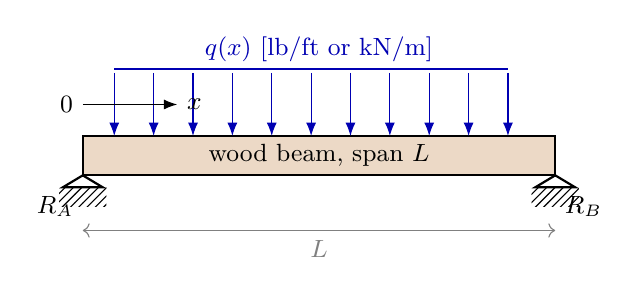
\begin{tikzpicture}[scale=1.0]

  % Ground hatching at supports
  \fill[pattern=north east lines] (-0.3,-0.4) rectangle (0.3,-0.15);
  \fill[pattern=north east lines] (5.7,-0.4) rectangle (6.3,-0.15);

  % Support triangles
  \draw[thick] (0,0) -- (-0.25,-0.15) -- (0.25,-0.15) -- cycle;
  \draw[thick] (6,0) -- (5.75,-0.15) -- (6.25,-0.15) -- cycle;

  % Beam body
  \draw[thick, fill=brown!30] (0,0) rectangle (6,0.5);
  \node at (3,0.25) {\small wood beam, span $L$};

  % Distributed load arrows (pointing down onto beam)
  \foreach \x in {0.4, 0.9, 1.4, 1.9, 2.4, 2.9, 3.4, 3.9, 4.4, 4.9, 5.4} {
    \draw[-Latex, blue!70!black] (\x, 1.3) -- (\x, 0.5);
  }
  % Load label
  \draw[blue!70!black] (0.4,1.35) -- (5.4,1.35);
  \node[blue!70!black] at (3, 1.6) {\small $q(x)$ [lb/ft or kN/m]};

  % Dimension line
  \draw[<->, gray] (0,-0.7) -- (6,-0.7) node[midway, below] {\small $L$};

  % Reaction labels
  \node[below left] at (0,-0.15) {\small $R_A$};
  \node[below right] at (6,-0.15) {\small $R_B$};

  % Coordinate axis
  \draw[-Latex] (0,0.9) -- (1.2,0.9) node[right] {\small $x$};
  \node at (0,0.9) [left] {\small $0$};

\end{tikzpicture}
\caption{Free-body diagram of the beam system. The system boundary encompasses the beam member between supports at $x=0$ and $x=L$. Distributed load $q(x)$ is applied externally from the surroundings. Reactions $R_A$ and $R_B$ represent the interaction with the supports.}
\label{fig:beam-fbd}
\end{figure}

The primary state variable is the \textbf{transverse deflection} $w(x)$, from which bending stress, shear stress, and the deflection-to-span ratio ($\delta/L$) are derived.

Key system parameters:
\begin{itemize}
  \item $E$ --- modulus of elasticity of the wood species/grade [psi or MPa]
  \item $I$ --- second moment of area of the cross-section [in$^4$ or mm$^4$]
  \item $L$ --- clear span of the member [ft or m]
  \item Cross-section dimensions: width $b$, depth $d$
\end{itemize}

% ---------------------------------------------------------------------------
\subsection{Surroundings}

The surroundings are everything external to the system that acts on it across the system boundary.
For a residential structural member, the surroundings consist of:

\begin{enumerate}
  \item \textbf{Applied distributed load $q(x)$} --- transferred from the floor or roof framing above through the wall plates and into the beam.
  This load has contributions from:
  \begin{itemize}
    \item Roof dead load (roofing, sheathing, framing): typically 10--15~psf
    \item Roof live load or snow load: 20--40~psf depending on climate zone
    \item Floor dead load: 10--15~psf
    \item Floor live load: 40~psf (residential occupancy per IRC)
    \item Tributary width $T_w$ [ft]: the width of roof/floor area carried by this member
  \end{itemize}
  The resultant line load is $q = (q_{\text{roof}} + q_{\text{floor}}) \times T_w$ [lb/ft].

  \item \textbf{Support reactions} --- the jack studs, posts, or bearing walls at $x = 0$ and $x = L$ provide the boundary conditions (pinned, fixed, or spring supports).

  \item \textbf{Gravity field} --- the gravitational body force is implicitly included in the load model above; no explicit body force term appears in the beam equation for transverse bending.
\end{enumerate}

Figure~\ref{fig:system-context} shows the system in context of a typical residential wall cross-section.

\begin{figure}[ht]
\centering
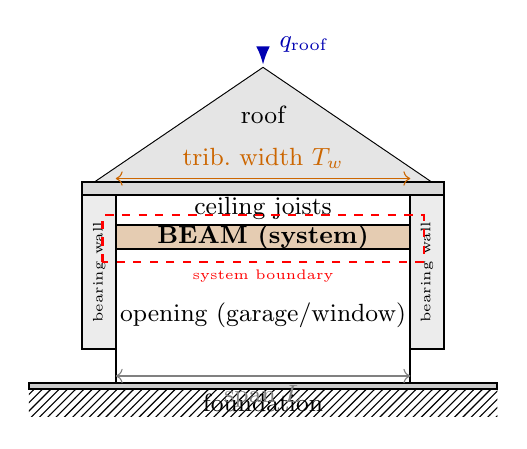
\begin{tikzpicture}[scale=0.85]

  % Roof triangle
  \draw[thick] (1,4.5) -- (3.5,6.2) -- (6,4.5);
  \fill[gray!20] (1,4.5) -- (3.5,6.2) -- (6,4.5) -- cycle;
  \node at (3.5,5.5) {\small roof};

  % Roof load arrow
  \draw[-Latex, blue!70!black, thick] (3.5,6.5) -- (3.5,6.25);
  \node[blue!70!black, right] at (3.6,6.55) {\small $q_{\text{roof}}$};

  % Ceiling/attic floor
  \draw[thick, fill=gray!30] (0.8,4.3) rectangle (6.2,4.5);
  \node at (3.5,4.1) {\small ceiling joists};

  % Left wall
  \draw[thick, fill=gray!15] (0.8,2.0) rectangle (1.3,4.3);
  \node[rotate=90] at (1.05, 3.15) {\tiny bearing wall};

  % Right wall
  \draw[thick, fill=gray!15] (5.7,2.0) rectangle (6.2,4.3);
  \node[rotate=90] at (5.95, 3.15) {\tiny bearing wall};

  % BEAM (system) highlighted
  \draw[thick, fill=brown!40] (1.3,3.5) rectangle (5.7,3.85);
  \node[font=\small\bfseries] at (3.5,3.675) {BEAM (system)};
  \draw[dashed, red, thick] (1.1,3.3) rectangle (5.9,4.0);
  \node[red, font=\tiny] at (3.5,3.1) {system boundary};

  % Opening below beam
  \draw[thick] (1.3,1.5) -- (1.3,3.5);
  \draw[thick] (5.7,1.5) -- (5.7,3.5);
  \node at (3.5,2.5) {\small opening (garage/window)};

  % Foundation
  \draw[thick, fill=gray!40] (0,1.4) rectangle (7,1.5);
  \fill[pattern=north east lines] (0,1.0) rectangle (7,1.4);
  \node at (3.5,1.2) {\small foundation};

  % Span dimension
  \draw[<->, gray] (1.3,1.6) -- (5.7,1.6) node[midway, below] {\small span $L$};

  % Tributary width annotation
  \draw[<->, orange!80!black] (1.3,4.55) -- (5.7,4.55) node[midway, above] {\small trib.\ width $T_w$};

\end{tikzpicture}
\caption{System in context. The beam (brown, highlighted by dashed red system boundary) spans an opening between bearing walls. Loads from the roof and ceiling framing above constitute the surroundings acting on the system. The tributary width $T_w$ determines how much roof area the beam carries.}
\label{fig:system-context}
\end{figure}

% ---------------------------------------------------------------------------
\subsection{Environments}

The \textbf{environment} defines the external conditions that determine parameter values and vary across use cases.
Three primary environments are relevant:

\begin{enumerate}
  \item \textbf{Geographic/Climatic Environment.}
  Snow and wind loads depend on location.
  A beam designed for a Virginia mountain site ($p_s = 40$~psf ground snow) requires different sizing than one in coastal Florida ($p_s = 0$~psf).
  The environment sets the load distribution parameters for uncertainty quantification.

  \item \textbf{Structural Context Environment.}
  Whether the member carries one-story, two-story, or roof-only loads changes the total tributary load.
  A header in a single-story garage differs from a girder in a two-story bearing wall.
  This determines whether $q_{\text{floor}}$ is zero or non-zero.

  \item \textbf{Material/Grade Environment.}
  Wood structural properties ($E$, $F_b$, $F_v$) vary by species and grade (e.g., Douglas Fir-Larch \#2 vs.\ Southern Yellow Pine \#1 vs.\ LVL engineered lumber).
  This is modeled as a random variable in the uncertainty quantification framework.
\end{enumerate}

Table~\ref{tab:environments} summarizes the key environments and their effect on model parameters.

\begin{table}[ht]
\centering
\caption{Environments and their effect on model parameters.}
\label{tab:environments}
\begin{tabular}{lll}
\toprule
\textbf{Environment} & \textbf{Variable affected} & \textbf{Range} \\
\midrule
Geographic (snow zone) & $q_{\text{snow}}$ & 0--60 psf \\
Structural context (story count) & $q_{\text{floor}}$ & 0 or 50--55 psf \\
Material grade & $E$, $F_b$, $F_v$ & see lumber tables \\
Tributary geometry & $T_w$ & 4--20 ft (typical residential) \\
\bottomrule
\end{tabular}
\end{table}

% =============================================================================
% SECTION 3: MATHEMATICAL MODEL (PDEs)
% =============================================================================

\section{Mathematical Model}

\subsection{Governing Equation}

The transverse deflection $w(x)$ of a beam subject to a distributed load $q(x)$ is governed by the \textbf{Euler--Bernoulli beam equation}:

\begin{equation}
  \frac{d^2}{dx^2}\!\left[ EI(x)\,\frac{d^2 w}{dx^2} \right] = q(x), \quad x \in (0, L)
  \label{eq:eb-general}
\end{equation}

For a prismatic member with uniform cross-section and homogeneous material, $EI$ is constant, and Eq.~\eqref{eq:eb-general} simplifies to:

\begin{equation}
  EI\,\frac{d^4 w}{dx^4} = q(x), \quad x \in (0, L)
  \label{eq:eb-prismatic}
\end{equation}

This is a linear, fourth-order ordinary differential equation---a 1D steady BVP in the single spatial coordinate $x$.

\subsection{Derived Quantities}

From the deflection field $w(x)$, the following quantities of engineering interest are derived:

\textbf{Bending moment:}
\begin{equation}
  M(x) = EI\,\frac{d^2 w}{dx^2}
  \label{eq:moment}
\end{equation}

\textbf{Shear force:}
\begin{equation}
  V(x) = EI\,\frac{d^3 w}{dx^3}
  \label{eq:shear}
\end{equation}

\textbf{Maximum bending stress} (at the extreme fiber, distance $c = d/2$ from neutral axis):
\begin{equation}
  \sigma_{\max} = \frac{M_{\max}\,c}{I} = \frac{M_{\max}}{S}
  \label{eq:bending-stress}
\end{equation}
where $S = I/c$ is the section modulus.

\textbf{Maximum shear stress} (rectangular cross-section):
\begin{equation}
  \tau_{\max} = \frac{3\,V_{\max}}{2\,A}
  \label{eq:shear-stress}
\end{equation}
where $A = b \cdot d$ is the cross-sectional area.

\subsection{Boundary Conditions}

The beam BVP requires four boundary conditions (two at each end) to close the fourth-order system.

\textbf{Simply-supported} (pin--pin), the standard IRC prescriptive assumption for headers:
\begin{equation}
  w(0) = 0, \quad \frac{d^2 w}{dx^2}\bigg|_{x=0} = 0, \qquad
  w(L) = 0, \quad \frac{d^2 w}{dx^2}\bigg|_{x=L} = 0
  \label{eq:bc-ss}
\end{equation}

\textbf{Fixed-fixed} (clamped--clamped), appropriate for engineered rim beams:
\begin{equation}
  w(0) = 0, \quad \frac{dw}{dx}\bigg|_{x=0} = 0, \qquad
  w(L) = 0, \quad \frac{dw}{dx}\bigg|_{x=L} = 0
  \label{eq:bc-ff}
\end{equation}

The simply-supported case~\eqref{eq:bc-ss} is used as the primary model for code verification because it admits a clean closed-form solution.

\subsection{Load Model}

For a uniform distributed load $q(x) = q_0$ (constant), the load is computed from the tributary area:
\begin{equation}
  q_0 = \bigl(q_{\text{roof}} + q_{\text{floor}}\bigr)\,T_w
  \label{eq:load}
\end{equation}
where $q_{\text{roof}}$ and $q_{\text{floor}}$ are area loads [psf] and $T_w$ is the tributary width [ft].

\subsection{Analytical Solution (Simply-Supported, Uniform Load)}

For the simply-supported beam under uniform load $q(x) = q_0$, integrating Eq.~\eqref{eq:eb-prismatic} four times with BCs~\eqref{eq:bc-ss} yields the exact closed-form solution:

\begin{equation}
  w(x) = \frac{q_0}{24EI}\Bigl(x^4 - 2L\,x^3 + L^3\,x\Bigr)
  \label{eq:exact-ss}
\end{equation}

The maximum deflection occurs at midspan $x = L/2$:
\begin{equation}
  w_{\max} = \frac{5\,q_0\,L^4}{384\,EI}
  \label{eq:wmax}
\end{equation}

The maximum bending moment occurs at midspan:
\begin{equation}
  M_{\max} = \frac{q_0\,L^2}{8}
  \label{eq:mmax}
\end{equation}

These exact solutions~\eqref{eq:exact-ss}--\eqref{eq:mmax} will serve as the benchmark for code verification in a future homework assignment.

\subsection{Performance Criteria}

The beam is considered \emph{structurally acceptable} if all three criteria are satisfied:

\begin{enumerate}
  \item \textbf{Bending stress:} $\sigma_{\max} \leq F_b$ (allowable bending stress for the lumber species/grade)
  \item \textbf{Shear stress:} $\tau_{\max} \leq F_v$ (allowable shear stress)
  \item \textbf{Deflection:} $w_{\max} \leq L/240$ (IRC serviceability limit)
\end{enumerate}

These criteria define the \emph{failure surface} in the uncertainty quantification framework.

% =============================================================================
% SECTION 4: NUMERICAL DISCRETIZATION
% =============================================================================

\section{Numerical Discretization Approach}

\subsection{Finite Difference Method}

The beam BVP~\eqref{eq:eb-prismatic} is discretized using the \textbf{finite difference method (FDM)}.
The domain $[0, L]$ is partitioned into $N$ equal sub-intervals of width $h = L/N$, yielding $N+1$ grid points:
\[
  x_i = i\,h, \quad i = 0, 1, \ldots, N
\]

The fourth-order derivative is approximated using the standard second-order central difference stencil:

\begin{equation}
  \frac{d^4 w}{dx^4}\bigg|_{x_i}
  \approx
  \frac{w_{i-2} - 4w_{i-1} + 6w_i - 4w_{i+1} + w_{i+2}}{h^4}
  + \mathcal{O}(h^2)
  \label{eq:fd-stencil}
\end{equation}

The discretized governing equation at each \emph{interior} point $i = 2, \ldots, N-2$ is:

\begin{equation}
  \frac{EI}{h^4}\Bigl(w_{i-2} - 4w_{i-1} + 6w_i - 4w_{i+1} + w_{i+2}\Bigr) = q_i
  \label{eq:fd-system}
\end{equation}

where $q_i = q(x_i)$ is the applied load at node $i$.

\subsection{Assembly into a Linear System}

Equation~\eqref{eq:fd-system} applied at all interior nodes yields a banded linear system:

\begin{equation}
  \mathbf{K}\,\mathbf{w} = \mathbf{f}
  \label{eq:linear-system}
\end{equation}

where $\mathbf{K} \in \mathbb{R}^{(N+1)\times(N+1)}$ is the stiffness matrix (pentadiagonal, bandwidth 5), $\mathbf{w}$ is the vector of unknown deflections, and $\mathbf{f}$ contains the load values scaled by $h^4/(EI)$.

\textbf{Simply-supported boundary conditions} are enforced as follows.
The Dirichlet conditions $w_0 = 0$ and $w_N = 0$ are imposed directly on rows 0 and $N$:
\begin{align}
  w_0 = 0 \quad &\Rightarrow \quad \text{row } 0: \; [1,\, 0,\, 0,\, \ldots] \\
  w_N = 0 \quad &\Rightarrow \quad \text{row } N: \; [\ldots,\, 0,\, 0,\, 1]
\end{align}

The zero-moment conditions $w''(0) = 0$ and $w''(L) = 0$ are handled via \textbf{ghost points}.
Applying the centered second-difference at each boundary with $w_0 = w_N = 0$:
\begin{align}
  \frac{w_{-1} - 2w_0 + w_1}{h^2} = 0 \;\wedge\; w_0 = 0
    \quad &\Rightarrow \quad w_{-1} = -w_1 \\
  \frac{w_{N-1} - 2w_N + w_{N+1}}{h^2} = 0 \;\wedge\; w_N = 0
    \quad &\Rightarrow \quad w_{N+1} = -w_{N-1}
\end{align}

These ghost-point values are substituted into the 5-point stencil at the \textbf{near-boundary nodes} $i = 1$ and $i = N-1$, yielding modified equations for rows 1 and $N-1$:
\begin{align}
  i = 1: &\quad \frac{EI}{h^4}\bigl(5w_1 - 4w_2 + w_3\bigr) = q_1
    \label{eq:fd-row1} \\
  i = N-1: &\quad \frac{EI}{h^4}\bigl(w_{N-3} - 4w_{N-2} + 5w_{N-1}\bigr) = q_{N-1}
    \label{eq:fd-rowNm1}
\end{align}
These modified stencils maintain $\mathcal{O}(h^2)$ consistency since the ghost-point approximation introduces only $\mathcal{O}(h^2)$ error in the moment condition.

The complete row structure of $\mathbf{K}$ is therefore:
\begin{itemize}
  \item Row 0: enforces $w_0 = 0$ (Dirichlet)
  \item Row 1: modified 3-term stencil from ghost-point substitution, Eq.~\eqref{eq:fd-row1}
  \item Rows 2 to $N-2$: standard 5-point stencil, Eq.~\eqref{eq:fd-system}
  \item Row $N-1$: modified 3-term stencil from ghost-point substitution, Eq.~\eqref{eq:fd-rowNm1}
  \item Row $N$: enforces $w_N = 0$ (Dirichlet)
\end{itemize}

The system~\eqref{eq:linear-system} is solved using a direct banded solver (LU factorization), exploiting the half-bandwidth-2 (5-diagonal) structure for $\mathcal{O}(N)$ cost.

\subsection{Grid Convergence}

The formal truncation error of stencil~\eqref{eq:fd-stencil} is second-order: $\tau = \mathcal{O}(h^2)$.
Therefore, as the mesh is refined ($N \to \infty$, $h \to 0$), the numerical solution converges to the exact solution at rate $p = 2$ in the $L^\infty$ norm:
\begin{equation}
  \|w_h - w_{\text{exact}}\|_\infty \propto h^2
  \label{eq:convergence}
\end{equation}

A grid convergence study will be performed in the code verification homework by computing the observed order of accuracy $\hat{p}$ from solutions on systematically refined grids ($h$, $h/2$, $h/4$) and comparing against the theoretical value $p = 2$.

\subsection{Uncertainty Quantification}

For uncertainty propagation, the linear solve is repeated $N_{\text{MC}}$ times with independently sampled load and material parameters:
\begin{align}
  T_w &\sim \text{Uniform}(T_{w,\min},\, T_{w,\max}) \quad &\text{(geometric ambiguity)} \\
  q_{\text{roof}} &\sim \mathcal{N}(\mu_{q,\text{roof}},\, \sigma_{q,\text{roof}}^2) \quad &\text{(code + variability)} \\
  q_{\text{floor}} &\sim \mathcal{N}(\mu_{q,\text{floor}},\, \sigma_{q,\text{floor}}^2) \\
  E &\sim \mathcal{N}(\mu_E,\, \sigma_E^2) \quad &\text{(wood grade variability)}
\end{align}

For each sample $j = 1, \ldots, N_{\text{MC}}$, the beam is solved and the performance criteria are evaluated.
The probability of failure is estimated as:
\begin{equation}
  \hat{P}_{\text{fail}} = \frac{1}{N_{\text{MC}}} \sum_{j=1}^{N_{\text{MC}}}
  \mathbf{1}\!\left(\sigma_{\max}^{(j)} > F_b \;\vee\; \tau_{\max}^{(j)} > F_v \;\vee\; w_{\max}^{(j)} > \frac{L}{240}\right)
  \label{eq:pfail}
\end{equation}

Since each FD solve completes in $\mathcal{O}(N)$ time and typical beam discretizations use $N = 50$--$500$ nodes, running $N_{\text{MC}} = 10{,}000$ Monte Carlo samples takes well under one second on modern hardware.
Also note that $L/240$ in the indicator function must be evaluated in the same units as $w_{\max}$ (inches).

\subsection{Summary}

Table~\ref{tab:numerical-summary} summarizes the numerical approach.

\begin{table}[ht]
\centering
\caption{Summary of numerical discretization choices.}
\label{tab:numerical-summary}
\begin{tabular}{ll}
\toprule
\textbf{Attribute} & \textbf{Choice} \\
\midrule
Governing equation & Euler--Bernoulli beam ODE (4th order, 1D) \\
Discretization method & Finite differences (FDM) \\
Spatial stencil & Central differences, $\mathcal{O}(h^2)$ \\
Linear solver & Banded LU factorization \\
Boundary conditions & Simply-supported (primary); fixed-fixed (secondary) \\
Typical grid size & $N = 100$--$500$ nodes \\
UQ method & Monte Carlo sampling ($N_{\text{MC}} = 10{,}000$) \\
Verification benchmark & Analytical solution, Eq.~\eqref{eq:exact-ss} \\
\bottomrule
\end{tabular}
\end{table}

% =============================================================================
% SECTION 5: VERIFICATION, VALIDATION, AND SUMMARY
% =============================================================================

\section{Verification and Validation Plans}

\subsection{Code Verification Plan}

Code verification confirms that the numerical solver correctly solves the mathematical model.
The primary approach is comparison against the analytical solution~\eqref{eq:exact-ss} for the simply-supported uniform-load case.

\begin{enumerate}
  \item \textbf{Point-wise comparison.}
  Compute $w_h(x_i) - w_{\text{exact}}(x_i)$ at all grid points and plot the error field.

  \item \textbf{Error norm calculation.}
  Compute the $L_2$ and $L_\infty$ norms of the discretization error:
  \[
    \|e\|_2 = \sqrt{h \sum_{i=0}^{N} \bigl(w_h(x_i) - w_{\text{exact}}(x_i)\bigr)^2},
    \qquad
    \|e\|_\infty = \max_i \bigl|w_h(x_i) - w_{\text{exact}}(x_i)\bigr|
  \]

  \item \textbf{Systematic mesh refinement.}
  Solve on a sequence of grids: $N = 10, 20, 40, 80, 160$ nodes.
  Plot $\|e\|_\infty$ vs.\ $h$ on a log--log scale and compute the observed order of accuracy:
  \[
    \hat{p} = \frac{\log\!\bigl(\|e\|_\infty^{(h)} / \|e\|_\infty^{(h/2)}\bigr)}{\log 2}
  \]
  The expected value is $\hat{p} \approx 2$, consistent with the $\mathcal{O}(h^2)$ central difference stencil.

  \item \textbf{Method of Manufactured Solutions (MMS).}
  To verify the solver for non-uniform loads and more general boundary conditions, a manufactured solution $w_{\text{mfg}}(x)$ is chosen (e.g., a polynomial or trigonometric function), and a source term $q_{\text{mfg}}(x) = EI\,w_{\text{mfg}}^{(4)}(x)$ is derived analytically.
  The solver is run with $q = q_{\text{mfg}}$ and the error against $w_{\text{mfg}}$ is computed and convergence verified.
\end{enumerate}

\subsection{Solution Verification Plan}

Solution verification establishes numerical uncertainty in the converged solution for a specific set of input parameters.

\begin{enumerate}
  \item Select a representative beam configuration (span, load, cross-section) representative of a typical residential header (e.g., $L = 8$~ft, $q_0 = 500$~lb/ft, $3.5'' \times 11.25''$ LVL).
  \item Compute solutions on three systematically refined grids ($h$, $h/2$, $h/4$).
  \item Apply the Grid Convergence Index (GCI) method (Roache) to estimate the discretization error in $w_{\max}$ and $\sigma_{\max}$.
  \item Establish a grid that achieves $< 0.1\%$ relative error in $w_{\max}$ while minimizing computational cost for subsequent MC runs.
\end{enumerate}

\subsection{Model Validation Plan}

Model validation confirms that the mathematical model (Euler--Bernoulli beam theory) correctly represents the real physical system.

\begin{enumerate}
  \item \textbf{Prescriptive code comparison.}
  For standard load scenarios (40~psf roof + 10~psf dead load), compare system-selected header sizes against IRC Table R602.7 span table prescriptions.
  Acceptance criterion: system recommendations match or are more conservative than IRC for $\geq 90\%$ of cases.

  \item \textbf{Serviceability limit validation.}
  Verify that computed $w_{\max}/L$ ratios for code-compliant assemblies remain below the IRC $L/240$ serviceability limit under the nominal design load.

  \item \textbf{Engineered design dataset.}
  A set of residential plan sets with stamped structural designs will serve as validation data.
  The true engineered header size should fall within the predicted feasible range for $\geq 80\%$ of cases.
\end{enumerate}

\subsection{Summary}

Table~\ref{tab:project-summary} summarizes the complete project setup.

\begin{table}[ht]
\centering
\caption{Semester project summary.}
\label{tab:project-summary}
\begin{tabular}{ll}
\toprule
\textbf{Item} & \textbf{Description} \\
\midrule
Application & Residential wood header/beam structural assessment \\
Real system & Horizontal wood member spanning a door/window opening \\
Model (PDE) & Euler--Bernoulli beam, 4th-order ODE, 1D steady BVP \\
Independent variable & $x \in [0, L]$ (position along beam axis) \\
State variable & $w(x)$ (transverse deflection) \\
Boundary conditions & Simply-supported (primary); fixed-fixed (secondary) \\
Numerical method & Finite differences, $\mathcal{O}(h^2)$ central stencil \\
Analytical solution & Available (uniform load, simply-supported) \\
UQ method & Monte Carlo ($N_{\text{MC}} = 10{,}000$ samples) \\
Team & Jason Cusati, Cheng-Shun Chuang \\
\bottomrule
\end{tabular}
\end{table}

This project is well-suited to the full VV\&UQ sequence: the governing equation is simple and tractable, an analytical solution exists for code verification, real-world validation data is accessible through building codes and stamped plans, and the fast beam solve enables large Monte Carlo campaigns for uncertainty quantification.


\end{document}
